\section{RESULTS: DEVELOPMENT DATA AND POWER}\label{ch:results}

This chapter reports what the development data (forecast days through 2019) show about where regime information helps, and how large an effect the design could reveal. In short, modelling volatility matters and switching correlations barely moves the loss. The results are descriptive: I examined ten ETF universes, ten regime definitions and two tail levels, and chose specifications after seeing them (Chapter~\ref{ch:data}). Each comparison states what it changes (Table~\ref{tab:differs}).

\subsection{How to read the tables}\label{sec:reading}

Every comparison reports the mean FZ0 difference $\bar d$ of the richer model minus the baseline, so a negative value favours the richer model, together with the HAC standard error, the two-sided 95\% interval, the two-sided $p$-value and the minimum detectable difference (MDE). A result inside the MDE is inconclusive for effects below the MDE; it does not show that the effect is absent. For scale, the smallest effect of interest of Section~\ref{sec:sesoi} is 0.002.

\subsection{Regime-specific volatility against a pooled normal}\label{sec:vol-results}

Giving each regime its own volatilities (model B) lowered the loss against the pooled normal A by 0.16 to 0.18 in three of the four ETF samples, about eighty to ninety times the smallest effect of interest, each with a two-sided $p$-value below 0.001, and by 0.11 in the fund sample (Table~\ref{tab:ladder-vol}). The exception is the main sample, SPY/IEF/GLD, where the estimate is $-0.0201$ (two-sided $p=0.408$) with an MDE of 0.0679, so its interval includes both a large improvement and none.

\begin{table}[t]
\centering\setstretch{1}\footnotesize\setlength{\tabcolsep}{5pt}
\caption{\uc{Regime-specific volatility against a pooled normal (B versus A)}}\label{tab:ladder-vol}
\begin{tabular}{lrrrcrrr}
\toprule
Sample & $n$ & $\bar d$ & SE & 95\% interval & $t$ & $p$ (2-sided) & MDE \\
\midrule
\multicolumn{8}{l}{\textbf{B versus A}}\\
SPY/IEF/GLD & 2,516 & $-$0.0201 & 0.0242 & [$-$0.0675, 0.0274] & $-$0.83 & 0.408 & 0.0679 \\
SPY/IEF/HYG & 1,944 & $-$0.1659 & 0.0373 & [$-$0.2390, $-$0.0929] & $-$4.45 & $<$0.001 & 0.1044 \\
Sectors & 2,516 & $-$0.1806 & 0.0252 & [$-$0.2300, $-$0.1312] & $-$7.17 & $<$0.001 & 0.0705 \\
Risk assets & 1,944 & $-$0.1586 & 0.0217 & [$-$0.2010, $-$0.1161] & $-$7.32 & $<$0.001 & 0.0607 \\
Funds 1992--2019 & 7,053 & $-$0.1057 & 0.0293 & [$-$0.1630, $-$0.0483] & $-$3.61 & $<$0.001 & 0.0820 \\
\bottomrule
\end{tabular}
\tabnote{Mean FZ0 difference $\bar d$ of the richer model minus the baseline over the forecast days, tail level $\alpha=5\%$, Gaussian chain, pooled mean; negative favours the richer model. SE: Bartlett-kernel HAC standard error. The interval is $\bar d\pm1.96\,\mathrm{SE}$. The $p$-value is two-sided. MDE $=2.8016\,\mathrm{SE}$ is the smallest true difference a two-sided 5\% test detects with 80\% power. Source: \texttt{output/explore/ladder/ladder\_dm\_table.csv}. Forecast days 2010--2019 (ETFs; credit and risk-asset samples start in 2012), 1992--2019 (funds).}
\end{table}


\subsection{A single-regime GARCH model class against static regime covariance}\label{sec:ladder-results}

The contrasts in Table~\ref{tab:ladder-margin} and Figure~\ref{fig:forest} replace block-constant regime volatilities by GARCH(1,1) volatilities. They compare model classes: the GARCH models have no regime dependence in volatility and also change the correlation input and the mean estimator (Table~\ref{tab:differs}). In the pre-declared family, RSC versus D in the four ETF samples, all four estimates are negative. After Holm's adjustment over the four, the adjusted $p$-values are 0.2341, 0.2341, 0.2247 and 0.0025, so the gate, which required significance in at least two samples, was met in one (the risk assets). The GARCH advantage is therefore suggestive, not established.

\begin{table}[t]
\centering\setstretch{1}\scriptsize\setlength{\tabcolsep}{5pt}
\caption{\uc{GARCH margins against static regime covariance}}\label{tab:ladder-margin}
\begin{tabular}{lrrrcrrrr}
\toprule
Sample & $n$ & $\bar d$ & SE & 95\% interval & $t$ & $p$ (2-sided) & MDE & Holm $p$ \\
\midrule
\multicolumn{8}{l}{\textbf{CCC versus B (non-nested)}}\\
SPY/IEF/GLD & 2,516 & $-$0.0247 & 0.0173 & [$-$0.0586, 0.0093] & $-$1.43 & 0.154 & 0.0485 \\
SPY/IEF/HYG & 1,944 & $-$0.0403 & 0.0269 & [$-$0.0931, 0.0125] & $-$1.49 & 0.135 & 0.0755 \\
Sectors & 2,516 & $-$0.0466 & 0.0235 & [$-$0.0926, $-$0.0006] & $-$1.99 & 0.047 & 0.0658 \\
Risk assets & 1,944 & $-$0.0803 & 0.0230 & [$-$0.1254, $-$0.0351] & $-$3.49 & $<$0.001 & 0.0645 \\
Funds 1992--2019 & 7,053 & $-$0.0315 & 0.0159 & [$-$0.0627, $-$0.0003] & $-$1.98 & 0.048 & 0.0446 \\
\midrule
\multicolumn{9}{l}{\textbf{RSC versus D (non-nested; pre-declared family)}}\\
SPY/IEF/GLD & 2,516 & $-$0.0259 & 0.0173 & [$-$0.0599, 0.0081] & $-$1.49 & 0.135 & 0.0486 & 0.2341 \\
SPY/IEF/HYG & 1,944 & $-$0.0406 & 0.0259 & [$-$0.0914, 0.0102] & $-$1.57 & 0.117 & 0.0726 & 0.2341 \\
Sectors & 2,516 & $-$0.0396 & 0.0223 & [$-$0.0832, 0.0040] & $-$1.78 & 0.075 & 0.0623 & 0.2247 \\
Risk assets & 1,944 & $-$0.0760 & 0.0222 & [$-$0.1195, $-$0.0325] & $-$3.43 & $<$0.001 & 0.0622 & \textbf{0.0025} \\
Funds 1992--2019 & 7,053 & $-$0.0306 & 0.0198 & [$-$0.0693, 0.0081] & $-$1.55 & 0.122 & 0.0554 & -- \\
\bottomrule
\end{tabular}
\tabnote{As Table~\ref{tab:ladder-vol}. Holm $p$: the pre-declared family is RSC versus D in the four ETF samples, Holm-adjusted over the four; the fund sample is not in the family. Bold: the one adjusted $p$-value below 0.05.}
\end{table}


\begin{figure}[p]
\centering
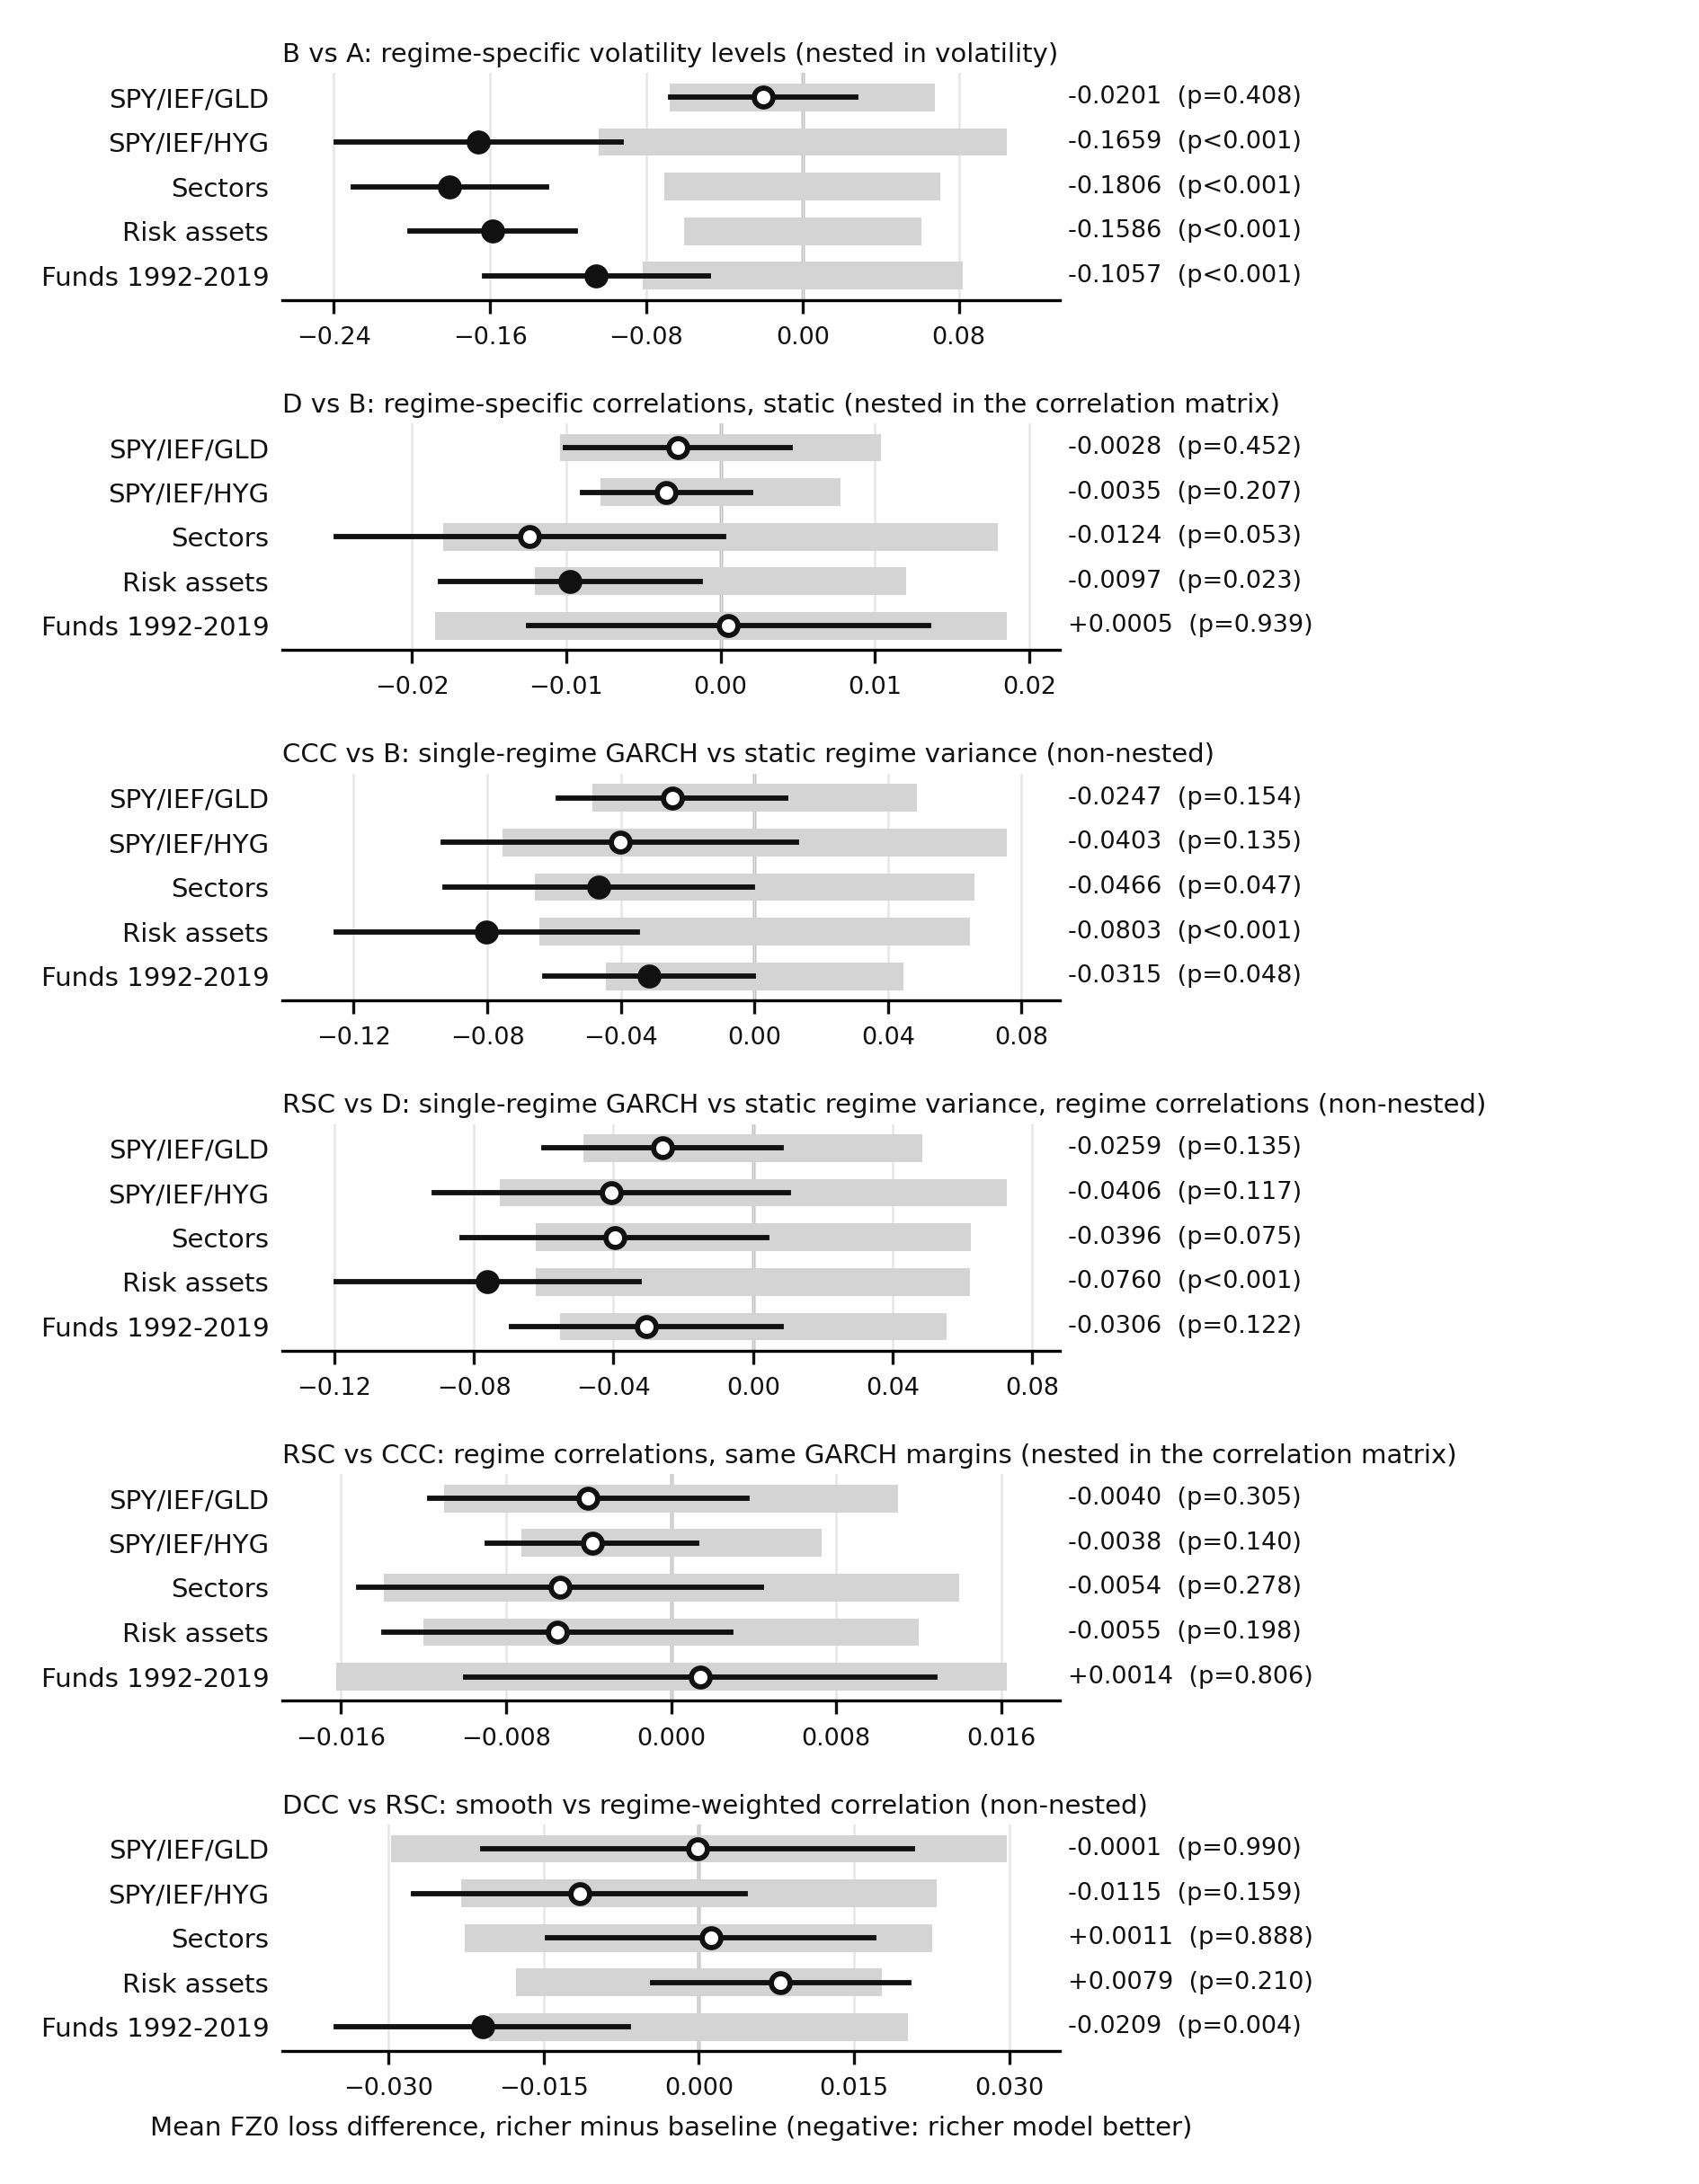
\includegraphics[width=\textwidth,height=0.84\textheight,keepaspectratio]{forest_comparisons_pooled.png}
\caption{\uc{Mean FZ0 difference, richer minus baseline, for each comparison and sample}}\label{fig:forest}
\tabnote{Points are $\bar d$; lines are two-sided 95\% intervals; the grey band is $\pm$ the MDE; filled points have a two-sided $p<0.05$ (unadjusted). Negative favours the richer model. Each panel has its own horizontal scale: the volatility and margin contrasts are roughly ten times larger than the correlation contrasts. Tail level 5\%, Gaussian chain, pooled mean. Source: \texttt{output/explore/ladder/ladder\_dm\_table.csv}, drawn by \texttt{scripts/thesis\_fig\_forest.py}.}
\end{figure}

The size of the contrast depends on the mean treatment, though not its sign. With a zero mean in both models the RSC-versus-D estimates range from $-0.0339$ to $-0.0814$, larger in absolute value than with the pooled mean; with regime-specific means they are close to the pooled ones ($-0.0263$ in the main sample; Appendix~\ref{app:mean}).

Calibration points the same way (Table~\ref{tab:hits}). On the ETF samples the static models overstate risk, with 5\% VaR breached on only 2.8\% to 4.2\% of days for A, B and D, while the GARCH-margin models breach it on 4.3\% to 5.5\%. In the fund sample the static models are close to nominal (B 5.4\%, D 5.3\%).

\begin{table}[t]
\centering\setstretch{1}\footnotesize\setlength{\tabcolsep}{5pt}
\caption{\uc{Share of days on which the return fell below the forecast VaR (nominal 5\%), development data}}\label{tab:hits}
\begin{tabular}{lrrrrrr}
\toprule
Sample & A & B & D & CCC & RSC & DCC \\
\midrule
SPY/IEF/GLD & 3.1\% & 3.7\% & 3.5\% & 5.0\% & 4.7\% & 5.0\% \\
SPY/IEF/HYG & 3.4\% & 4.2\% & 4.0\% & 5.5\% & 5.5\% & 5.0\% \\
Sectors & 3.1\% & 3.4\% & 3.7\% & 5.2\% & 5.4\% & 5.5\% \\
Risk assets & 2.8\% & 2.8\% & 3.0\% & 4.3\% & 4.6\% & 4.7\% \\
Funds 1992--2019 & 4.8\% & 5.4\% & 5.3\% & 5.5\% & 5.2\% & 5.5\% \\
\bottomrule
\end{tabular}
\tabnote{Gaussian chain, pooled mean, forecast days as in Table~\ref{tab:ladder-vol}. A hit is a day with $y_t\le\mathrm{VaR}_t$. Source: \texttt{output/explore/ladder/ladder\_loss\_table.csv}.}
\end{table}


\subsection{The correlation steps}\label{sec:corr-results}

Letting correlations switch, with the volatility model held fixed, never improved the loss detectably (Table~\ref{tab:ladder-corr}). With GARCH margins, switching all correlations (RSC versus CCC) gives estimates between $-0.0040$ and $-0.0055$ in the four ETF samples and $+0.0014$ in the funds; every interval includes zero (two-sided $p$-values from 0.140 to 0.806), and the estimates are between about a third and a half of their MDEs (0.36 to 0.52). The data are consistent with gains up to about the MDE. The answer is not the same under every mean treatment: with a zero mean the sector sample gives $-0.0087$ (two-sided $p=0.046$, unadjusted) and the risk-asset sample $-0.0070$ ($p=0.080$). The smooth alternative, DCC, is indistinguishable from RSC in the ETF samples ($p$ from 0.159 to 0.990) and better than RSC in the fund sample by $0.0209$ ($p=0.004$, unadjusted).

\begin{table}[t]
\centering\setstretch{1}\footnotesize\setlength{\tabcolsep}{5pt}
\caption{\uc{Correlation steps}}\label{tab:ladder-corr}
\begin{tabular}{lrrrcrrr}
\toprule
Sample & $n$ & $\bar d$ & SE & 95\% interval & $t$ & $p$ (2-sided) & MDE \\
\midrule
\multicolumn{8}{l}{\textbf{D versus B (nested in the correlation matrix; size unreliable under GARCH margins)}}\\
SPY/IEF/GLD & 2,516 & $-$0.0028 & 0.0037 & [$-$0.0101, 0.0045] & $-$0.75 & 0.452 & 0.0104 \\
SPY/IEF/HYG & 1,944 & $-$0.0035 & 0.0028 & [$-$0.0089, 0.0019] & $-$1.26 & 0.207 & 0.0078 \\
Sectors & 2,516 & $-$0.0124 & 0.0064 & [$-$0.0249, 0.0002] & $-$1.93 & 0.053 & 0.0179 \\
Risk assets & 1,944 & $-$0.0097 & 0.0043 & [$-$0.0182, $-$0.0013] & $-$2.27 & 0.023 & 0.0120 \\
Funds 1992--2019 & 7,053 & 0.0005 & 0.0066 & [$-$0.0125, 0.0135] & 0.08 & 0.939 & 0.0185 \\
\midrule
\multicolumn{8}{l}{\textbf{RSC versus CCC (nested in the correlation matrix)}}\\
SPY/IEF/GLD & 2,516 & $-$0.0040 & 0.0039 & [$-$0.0117, 0.0037] & $-$1.02 & 0.305 & 0.0110 \\
SPY/IEF/HYG & 1,944 & $-$0.0038 & 0.0026 & [$-$0.0089, 0.0013] & $-$1.48 & 0.140 & 0.0073 \\
Sectors & 2,516 & $-$0.0054 & 0.0050 & [$-$0.0151, 0.0044] & $-$1.08 & 0.278 & 0.0139 \\
Risk assets & 1,944 & $-$0.0055 & 0.0043 & [$-$0.0139, 0.0029] & $-$1.29 & 0.198 & 0.0120 \\
Funds 1992--2019 & 7,053 & 0.0014 & 0.0058 & [$-$0.0099, 0.0128] & 0.25 & 0.806 & 0.0162 \\
\midrule
\multicolumn{8}{l}{\textbf{DCC versus RSC (non-nested)}}\\
SPY/IEF/GLD & 2,516 & $-$0.0001 & 0.0106 & [$-$0.0209, 0.0207] & $-$0.01 & 0.990 & 0.0297 \\
SPY/IEF/HYG & 1,944 & $-$0.0115 & 0.0082 & [$-$0.0276, 0.0045] & $-$1.41 & 0.159 & 0.0229 \\
Sectors & 2,516 & 0.0011 & 0.0081 & [$-$0.0147, 0.0169] & 0.14 & 0.888 & 0.0226 \\
Risk assets & 1,944 & 0.0079 & 0.0063 & [$-$0.0045, 0.0203] & 1.25 & 0.210 & 0.0177 \\
Funds 1992--2019 & 7,053 & $-$0.0209 & 0.0072 & [$-$0.0351, $-$0.0068] & $-$2.90 & 0.004 & 0.0202 \\
\bottomrule
\end{tabular}
\tabnote{As Table~\ref{tab:ladder-vol}.}
\end{table}


The static step D versus B needs a caution. Under the simulated process with GARCH margins and no change in correlation (scenario S0), the one-sided test of D against B rejects in 9.6\% of replications (95\% interval 7.0\% to 12.2\%) at 1,508 test days, in 11.0\% (6.7\% to 15.3\%) at 2,520 days, and in 14.8\% and 17.0\% of replications at $|t|>1.96$ (Table~\ref{tab:power1508}). The test is oversized when volatility clusters. In the exploration grid, 37 of the 214 headline D-versus-B tests have a raw $p<0.05$ (17.3\%), 18 favouring D and 19 favouring B, and none survives a Holm adjustment (smallest adjusted $p=0.1413$). That rate matches the simulated null rate, so the raw count is not evidence of an effect. The simulated process is stylised and the 214 tests are not independent, so the match is suggestive, not proof.

\subsection{The primary pair on the development data}\label{sec:pair-dev}

On the development data the confirmatory comparison, RSC\_P against CCC, gives an estimate of $-0.0015$ over 2010 to 2019 (two-sided $p=0.136$, MDE 0.0028), $-0.0012$ in 2010--2015 ($p=0.371$) and $-0.0019$ in the dry-run years 2016--2019 ($p=0.198$; Table~\ref{tab:real-pair}). These estimates are about the size of the smallest effect of interest and not significant. Their standard errors, $0.0010$, $0.0013$ and $0.0015$, are the ones relevant to the hold-out, which has 1,508 days. Because the pair, the model and the test were chosen with these days in view, they validate nothing.

\begin{table}[t]
\centering\setstretch{1}\footnotesize\setlength{\tabcolsep}{3.5pt}
\caption{\uc{Single-pair correlation switching against constant correlation, development data (RSC\_P versus CCC)}}\label{tab:real-pair}
\begin{tabular}{llrrrcrrr}
\toprule
$\alpha$ & Forecast days & $n$ & $\bar d$ & SE & 95\% interval & $t$ & $p$ (2-sided) & MDE \\
\midrule
5.0\% & 2010--2019 & 2,516 & $-$0.0015 & 0.0010 & [$-$0.0034, 0.0005] & $-$1.49 & 0.136 & 0.0028 \\
5.0\% & 2010--2015 & 1,510 & $-$0.0012 & 0.0013 & [$-$0.0038, 0.0014] & $-$0.89 & 0.371 & 0.0037 \\
5.0\% & 2016--2019 & 1,006 & $-$0.0019 & 0.0015 & [$-$0.0048, 0.0010] & $-$1.29 & 0.198 & 0.0041 \\
2.5\% & 2010--2019 & 2,516 & $-$0.0028 & 0.0015 & [$-$0.0058, 0.0002] & $-$1.82 & 0.069 & 0.0043 \\
2.5\% & 2010--2015 & 1,510 & $-$0.0029 & 0.0021 & [$-$0.0070, 0.0012] & $-$1.37 & 0.171 & 0.0059 \\
2.5\% & 2016--2019 & 1,006 & $-$0.0027 & 0.0022 & [$-$0.0070, 0.0017] & $-$1.20 & 0.231 & 0.0062 \\
\bottomrule
\end{tabular}
\tabnote{RSC\_P minus CCC, Gaussian chain, pooled mean; negative favours switching the SPY--IEF correlation. SE is MDE$/2.8$ (the table stores MDE rounded to $2.8\,\mathrm{SE}$); the interval is $\bar d\pm1.96\,\mathrm{SE}$. These are development data: the specification was chosen after seeing them, so they are not validation. Source: \texttt{output/explore/routes/routes\_dm\_table.csv}, provider HMM\_SPY2.}
\end{table}


\subsection{Power at the hold-out length}\label{sec:power-results}

At 1,508 test days the primary test is correctly sized and has low power (Table~\ref{tab:power1508}). Its size, the rejection rate in S0, is 3.6\% (95\% interval 2.0\% to 5.2\%), so there is no sign of oversizing, although 500 replications cannot show that the size is at most 5\%; the mean difference in S0 is slightly positive, so the null is interior and not on the boundary. The power is 18.2\% (14.8\% to 21.6\%) in the moderate scenario S1, 35.2\% (31.0\% to 39.4\%) in the strong scenario S2 and 2.4\% in the flight-to-quality scenario S3, where correlations move the other way. At 2,520 test days the corresponding one-sided power was 27.0\% and 53.5\%, so the shorter hold-out costs substantial power. The pre-declared low-power rule, which would have made the hold-out chapter open by saying that the test cannot be expected to detect any simulated shift, applied if S2 power fell below 30\%; at 35.2\% it does not apply, but a moderate shift would be detected about one time in five.

\begin{table}[t]
\centering\setstretch{1}\footnotesize\setlength{\tabcolsep}{3.5pt}
\caption{\uc{Simulated size and power of the difference tests (500 replications per scenario at 1,508 days; 200 at 2,520 days)}}\label{tab:power1508}
\begin{tabular}{lcccrr}
\toprule
Scenario & One-sided rejection [95\% CI] & Two-sided & Upper tail & Mean $\bar d$ & Mean SE \\
\midrule
\multicolumn{6}{l}{\textbf{Primary test: RSC\_P versus CCC, 1,508 test days, 500 replications}}\\
S0 (no correlation change) & 3.6\% [2.0\%, 5.2\%] & 7.4\% & 5.2\% & 0.0002 & 0.0006 \\
S1 (moderate) & 18.2\% [14.8\%, 21.6\%] & 14.2\% & 0.4\% & $-$0.0009 & 0.0010 \\
S2 (strong) & 35.2\% [31.0\%, 39.4\%] & 24.2\% & 0.0\% & $-$0.0034 & 0.0026 \\
S3 (flight to quality) & 2.4\% [1.1\%, 3.7\%] & 4.8\% & 3.4\% & 0.0002 & 0.0017 \\
\midrule
\multicolumn{6}{l}{\textbf{Same test, 2,520 test days (earlier study, 200 replications)}}\\
S0 (no correlation change) & 4.5\% [1.6\%, 7.4\%] & 7.0\% & 4.5\% & 0.0001 & 0.0005 \\
S1 (moderate) & 27.0\% [20.8\%, 33.2\%] & 17.5\% & 0.0\% & $-$0.0009 & 0.0008 \\
S2 (strong) & 53.5\% [46.6\%, 60.4\%] & 44.0\% & 0.0\% & $-$0.0035 & 0.0020 \\
S3 (flight to quality) & 5.5\% [2.3\%, 8.7\%] & 3.5\% & 1.0\% & 0.0001 & 0.0013 \\
\midrule
\multicolumn{6}{l}{\textbf{RSC versus CCC (all pairs switch), 1,508 test days}}\\
S0 (no correlation change) & 4.6\% [2.8\%, 6.4\%] & 7.2\% & 4.2\% & 0.0004 & 0.0018 \\
S1 (moderate) & 17.2\% [13.9\%, 20.5\%] & 9.8\% & 0.4\% & $-$0.0022 & 0.0032 \\
S2 (strong) & 25.4\% [21.6\%, 29.2\%] & 17.0\% & 0.0\% & $-$0.0069 & 0.0069 \\
S3 (flight to quality) & 2.6\% [1.2\%, 4.0\%] & 6.6\% & 5.2\% & 0.0010 & 0.0036 \\
\midrule
\multicolumn{6}{l}{\textbf{Static D versus B, 1,508 test days (size under GARCH margins)}}\\
S0 (no correlation change) & 9.6\% [7.0\%, 12.2\%] & 14.8\% & 8.0\% & 0.0002 & 0.0024 \\
\bottomrule
\end{tabular}
\tabnote{Tail level $\alpha=5\%$, Gaussian chain, simulated data from the stylised GARCH regime-switching process (Section~\ref{sec:power-design}); S0 is the null and its row is the test size. One-sided: reject when $t<-1.6449$ (the pre-declared rule). Two-sided: $|t|>1.96$. Upper tail: $t>+1.96$, the rate at which the richer model is declared significantly worse. The interval is a 95\% binomial interval on the replications. Mean $\bar d$ and mean SE are averages over replications. Sources: \texttt{power\_1508\_summary.csv}, \texttt{power\_2520\_twosided.csv}.}
\end{table}


Simulated power does not transfer one-for-one to the real data. The mean standard error of the primary difference in the simulation depends on the scenario: it is 0.0006 in S0, 0.0010 in S1 and 0.0026 in S2, because a larger shift in correlation makes the loss difference more variable. The real-data standard errors above, 0.0010 to 0.0015, lie between the S0 and S2 values, so the power of 35.2\% in S2 reflects both a mean difference of $-0.0034$ and a standard error of 0.0026, and it is not the power that the same difference would have on real data. The minimum detectable difference at the real standard error, about $2.4865\times0.0014=0.0035$ for the one-sided test (0.0031 at the standard error observed on the hold-out, Chapter~\ref{ch:holdout}), is the more transferable summary.
